\section{Results and discussion}\label{sec:result}
We will now first take a look at the case of two electrons in a potential with different oscillator energies. In order to do so, we perform a Variational Monte Carlo simulation and use the Metropolis algorithm explained in section~\ref{sec:metropolis} to find the energy of the ground state. Therefore we use numerical derivation. We will later introduce analytical calculations based on closed-form expressions as well (section~\ref{sec:analytical}). Besides, we put emphasis on the correlations introduced by the Jastrow factor by computing the kinetic and potential energy of the ground state for different oscillator frequencies.\\
In addition we introduce importance sampling and analyse the dependency of the results to the time step $\delta t$.\\
\subsection{Two electron case}\label{sec:2electron}
Since it is the easiest case, we first look at two electrons in a quantum dot interacting with each other. According to \cite{lohne2011} the corresponding energy is at $E = 3$.\\
For the computation we use the variational wave function
\begin{equation}
\psi_T(\mathbf{r_1,r_2}) = C \exp\left[-\alpha\frac{\omega}{2} (r_1^2+r_2^2)\right] \exp \left[ \frac{a_{12} r_{12}}{(1+\beta r_{12})} \right],
\end{equation}
where we start by considering a wide range of $\alpha \in[0.7,1.3]$ and $\beta \in[0.2,0.6]$ first and perform a more precise simulation afterwards. The goal is to find the variational parameters $\alpha$ and $\beta$, where the energy is at its minimum. After the first simulation we notice, that the minimum must be somewhere around $\alpha \in[0.9,1.1]$ and $\beta \in[0.35,0.45]$. This is why we preform a simulation with these boundaries and use 12 000 000 Metropolis cycles to get an accurate result. In figure~\ref{fig:2electron} the energy is plotted depending on both variational parameters $\alpha$ and $\beta$. The 3D-plot results in a bended plane resembling to the shape of a valley. For increasing $\alpha$ the corresponding $\beta$ at minimal energy is decreasing. The minimum energy calculated is 
\begin{align}
E &= 3.0003
\intertext{at}
\alpha &= 0.9867,\\
\beta &= 0.4033
\intertext{and at a mean electron distance of}
r_{12} &=1.607
\end{align}
As mentioned before we were expecting the energy to be at $E=3$, so the calculated value matches the expected one very well. In figure~\ref{fig:2electron} there are some areas, where the plane is not as smooth as in others. We classify these small perturbations to the valley as numerical fluctuations and consider them to be less important.\\
To get a better understanding of the influence the parameters have on the calculated energy, figure~\ref{fig:2electronalpha} shows the energy's $\alpha$-dependency for different $\beta$. Consistent with figure~\ref{fig:2electron} this figure reveals, that $\beta$ is shifted depending on $\alpha$ and that $\alpha$ has a larger influence on the energy than the other variational parameter. The errors plotted in figure~\ref{fig:2electronalpha} are almost invisible, since they are very small compared to the energy fluctuations at varying $\alpha$ and $\beta$. In figure~\ref{fig:VMCfein} we also show the energy minimum dependent on $\beta$. In this plot, the errors seem to be larger, but in order to find the minimum, we had to look at a very small energy scale. Overall there are not many cases, where the error is significantly high, so we consider our results to be of sufficient accuracy.
\begin{figure}[htbp]
    \centering
    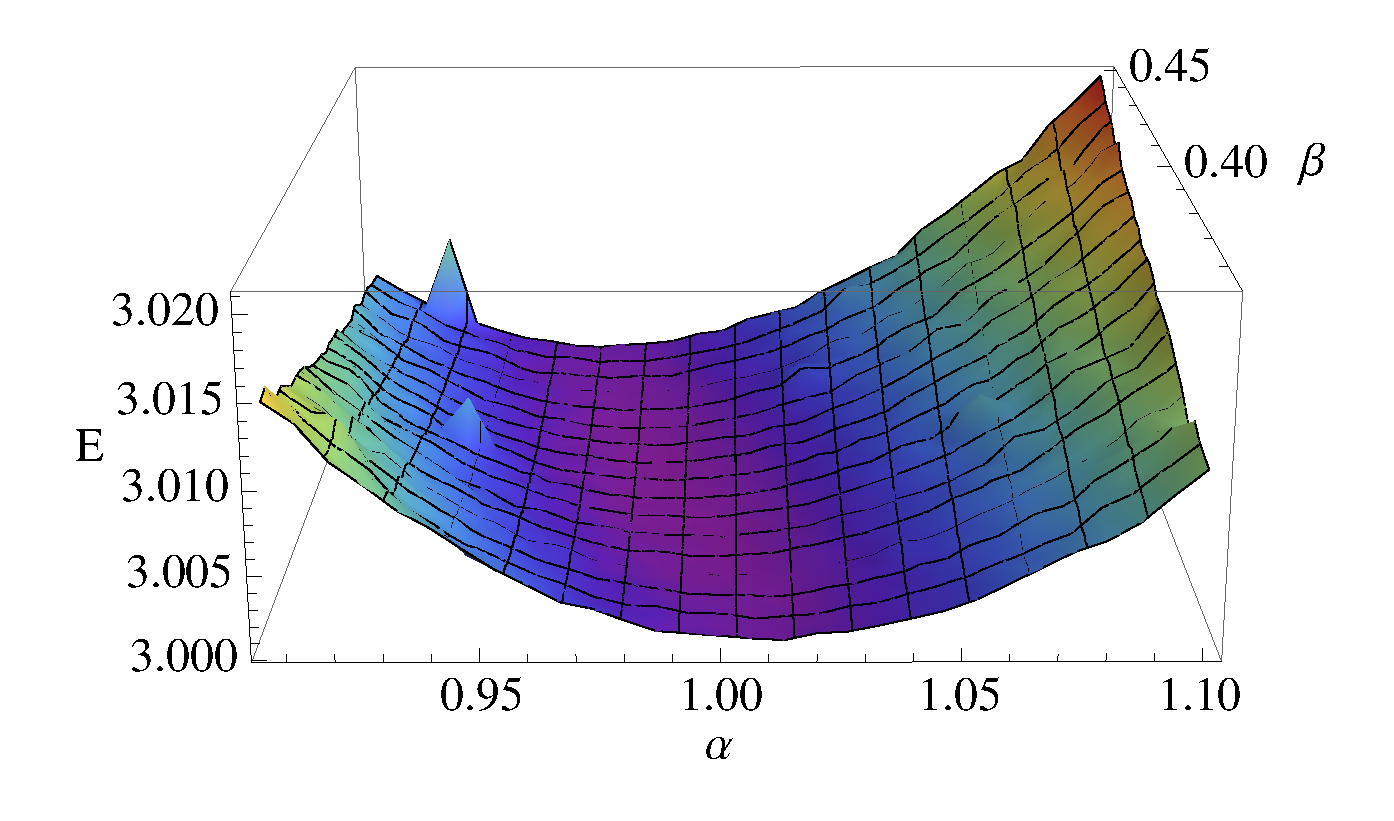
\includegraphics[scale=0.45]{2electron}
    \caption{Plot of $\alpha$- and $\beta$-dependencies of the ground state energy for two interacting electrons at the ground state based on a simulation involving 12 000 000 Metropolis cycles}
    \label{fig:2electron}
\end{figure}
\begin{figure}[htbp]
    \centering
    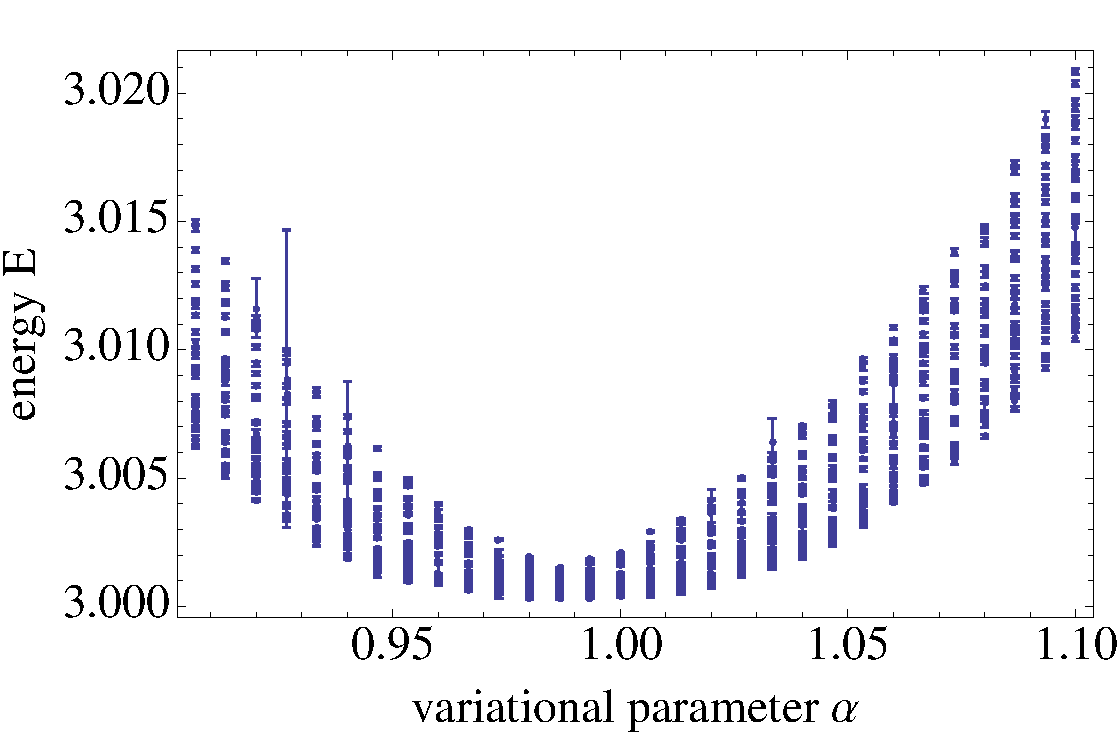
\includegraphics[scale=0.45]{2electronalpha}
    \caption{Plot of $\alpha$-dependency of the ground state energy for two interacting electrons at the ground state for different $\beta$ based on a simulation involving 12 000 000 Metropolis cycles}
    \label{fig:2electronalpha}
\end{figure}
\begin{figure}[htbp]
    \centering
    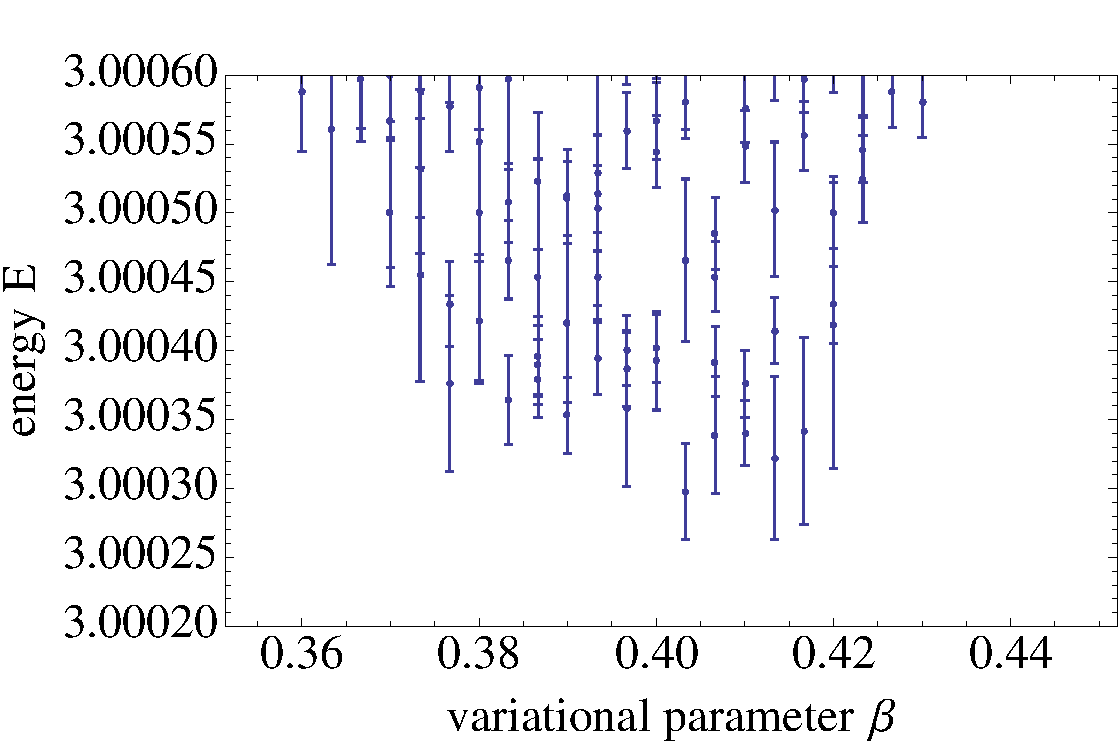
\includegraphics[scale=0.45]{VMCfein}
    \caption{Plot of $\beta$-dependency of the ground state energy for two interacting electrons at the ground state for different $\alpha$ based on a simulation involving 12 000 000 Metropolis cycles}
    \label{fig:VMCfein}
\end{figure}
\FloatBarrier
\subsubsection{Jastrow factor}\label{sec:Jastro}
After computing the ground state energy we now analyse the changement in energy arising from different osciallator potentials $\omega$. The corresponding 3D-plots with the $\alpha$-$\beta$-dependency of the energy can be found in Appendix~\ref{sec:appendix}. The results for $\omega =\{1.00, 0.70, 0.50,0.28,0.01\}$ are shown in table~\ref{tab:omega}. It can be observed, that for small oscillator frequency the kinetic energy drops relative to the total energy of the system. The reason for this is, that for small $\omega$ the potential gets wider, but flatter as well. In this case, the electrons interact less with each other, because they are further apart. As a result, kinetic energy drops.\\
\begin{table}[H]
\centering
\caption{Kinetic and potential energy depending on the oscillator frequency $\omega$}
    \begin{tabular}{c|cc|c|c|c}
   \toprule
    $\omega$ & $E_{kin}$  & $E_{pot}$  & $E_{kin} (\%)$ & $E_{total}$ & $E_{\citep{hogberget2013}}$ \\ 
    \midrule
    0.01   & 0.010 & 0.064 & 14   & 0.074    & 0.074   \\
    0.28   & 0.248  & 0.773  & 24   & 1.021   & 1.022  \\
    0.50    & 0.452  & 1.206   & 27   & 1.658  & 1.660    \\
    0.70    & 0.607  & 1.600   & 28   &  2.207    & -   \\
    1.00      & 0.862  & 2.137   & 29   & 3.0003  & 3.0003    \\
    \bottomrule
    \end{tabular}
\label{tab:omega}
\end{table}
In the wave equation
\begin{equation}
\psi_T(\mathbf{r_1,r_2}) = C \exp\left[-\alpha\frac{\omega}{2} (r_1^2+r_2^2)\right] \exp \left[ \frac{a_{12} r_{12}}{(1+\beta r_{12})} \right]
\end{equation}
only the first exponential term is affected by the oscillator frequency $\omega$, while the Jastrow factor does not contain the frequency.\\
For vanishing potential as for $\omega =0.01$ the wave function becomes:
\begin{equation}
\lim_{\omega\rightarrow 0} \psi_T(\mathbf{r_1,r_2}) = C \exp \left[ \frac{a_{12} r_{12}}{(1+\beta r_{12})} \right] = C J,
\end{equation}
where $J$ is the Jastrow factor. This means, that in this case the Jastrow factor adopts a more important role. The interaction potential is then compared to the oscillator potential at a higher value.
\subsubsection{Importance sampling: $\delta t$-dependency}
To obtain accurate results we also introduce important sampling and optimize the calculation of the energy by studying its time step dependency. We will refer to the time step as $\delta t$. The time step plays an important role in importance sampling, since it the biasing when calculating new random numbers. For large $\delta t$ the newly picked random numbers for the particle position can vary more, than for smaller $\delta t$. It is therefore relevant to use a reasonable time step to aviod jumping to far in the position or to get stuck in one place as explained previously in section~\ref{sec:importance}. In figure~\ref{fig:importance} we plotted the energy calculated for $\alpha = 0.98$ and $\beta = 0.40$ (according to~\ref{sec:2electron}) for diverse $\delta t$. Comparing the results including importance sampling to those in section~\ref{sec:2electron} we notice, that with importance sampling we can obtain a lot smaller energies, than when using a brute force Metropolis algorithm. This shows, that the importance sampling has an impact on the precision of the results, because we get energies very near the exact solution.\\
Concerning the optimal value of $\delta t$, it is obvious in figure~\ref{fig:importance}, that it must be $\delta t \in [0.1,0.2]$. Because of the statistical spread of the energy values, we cannot find the one and only perfect $\delta t$-value. For large time steps, that are still smaller than $\delta t= 4$ the energy converges to $E=3.002$. For even higher time steps, the calculated energy increases strongly and precise simulations become impossible.\\
For further simulations we will vary the time step depending on the oscillator freuqency as well, because of the potential spread for small frequencies. In this case, we have to higher the time step to get stable importance sampling with enough accepted steps. Otherwise we might end up as described in section~\ref{sec:importance} at the boundaries of our distribution or in a small intervall at a certain point, producing biased data.
\begin{figure}[htbp]
    \centering
    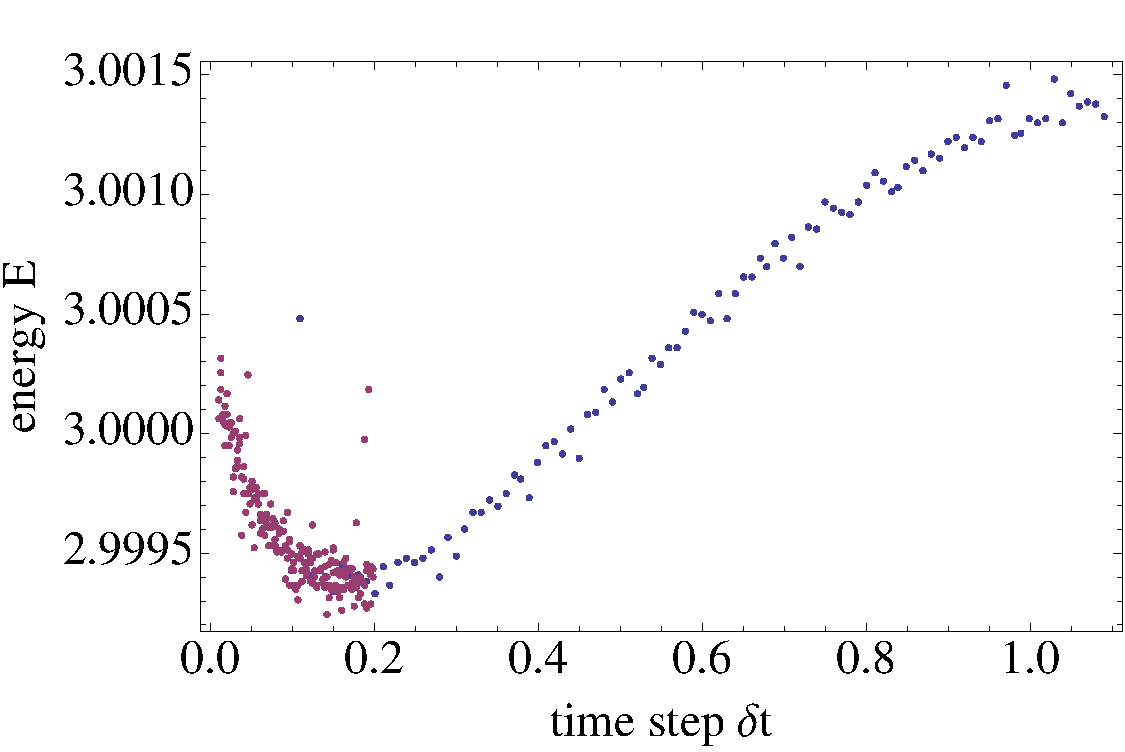
\includegraphics[scale=0.6]{importance}
    \caption{Results of energy calculation for varying time steps $\delta t$ in the importance sampling. The blue dots refer to a wide-spaced simulation for $\delta t \in [0.1,1]$ with step length $\Delta (\delta t) = 0.01$, whereas the violet dots refer to $\delta t\in [0.01,0.2]$ with $\Delta(\delta t) = 0.001$}
    \label{fig:importance}
\end{figure}
\FloatBarrier


\subsection{Six electron case}\label{sec:6electron}
In this part we introduce the six electron case. In order to do so we consider the more general trial wave function \ref{glg:sixelectron} which also can be reduced to the case of two electrons. The simulations are done like in section \ref{sec:2electron} but with $400000$ cycles, because of higher computation times. These are devided on 4 threads. For the time-step of the importance sampling (eq. \ref{eq:quantum_force}) we use the value $\delta t = 0.5$ for small oscillator frequencies and smaller time steps for higher frequencies ($\delta t = 0.1$ for $\omega = 1$). 

\subsubsection{Perturbed case}\label{sec:perturbed_six}
For the perturbed six electron system the ground state energies are shown in table \ref{tab:groundstate_sixelectron}. Comparing the energies with \citet{hogberget2013} or alternatively with \citet{lohne2011} we have a good agreement for the values. For increasing $\omega$ we have higher values of $\alpha$ and $\beta$. Figure \ref{fig:alpha_beta_omega} shows the dependencies in this case. It can be seen that there is no easy linear coherence, instead we made an arbitrarily chosen fit with a square-root function which seemed for us the best approximation and deals as a reference where to search for the energy minima for different $\omega$. 
\begin{table}
    \centering
    \caption{Ground state energies for six electrons in an oscillator well.}
    \begin{tabular}{c|cc|c|c}
    \toprule
    $\omega$   & $\alpha$    & $\beta$ &    $E$  & $E_{\citep{hogberget2013}}$  \\ 
    \midrule
    $0.01$     & $0.700$       & $0.08$  & $0.6986$ & - \\
    $0.28$     & $0.800$       & $0.25$  & $7.7360$  & 7.6216 \\
    $0.50$      & $0.925$	    & $0.38$  & $11.8047$ & 11.8103 \\
    $1.00$     & $0.980$      & $0.45$  & $20.1850$ & 20.1902 \\
    \bottomrule
    \end{tabular}
    \label{tab:groundstate_sixelectron}
\end{table}
\begin{figure}[htbp]
    \centering
    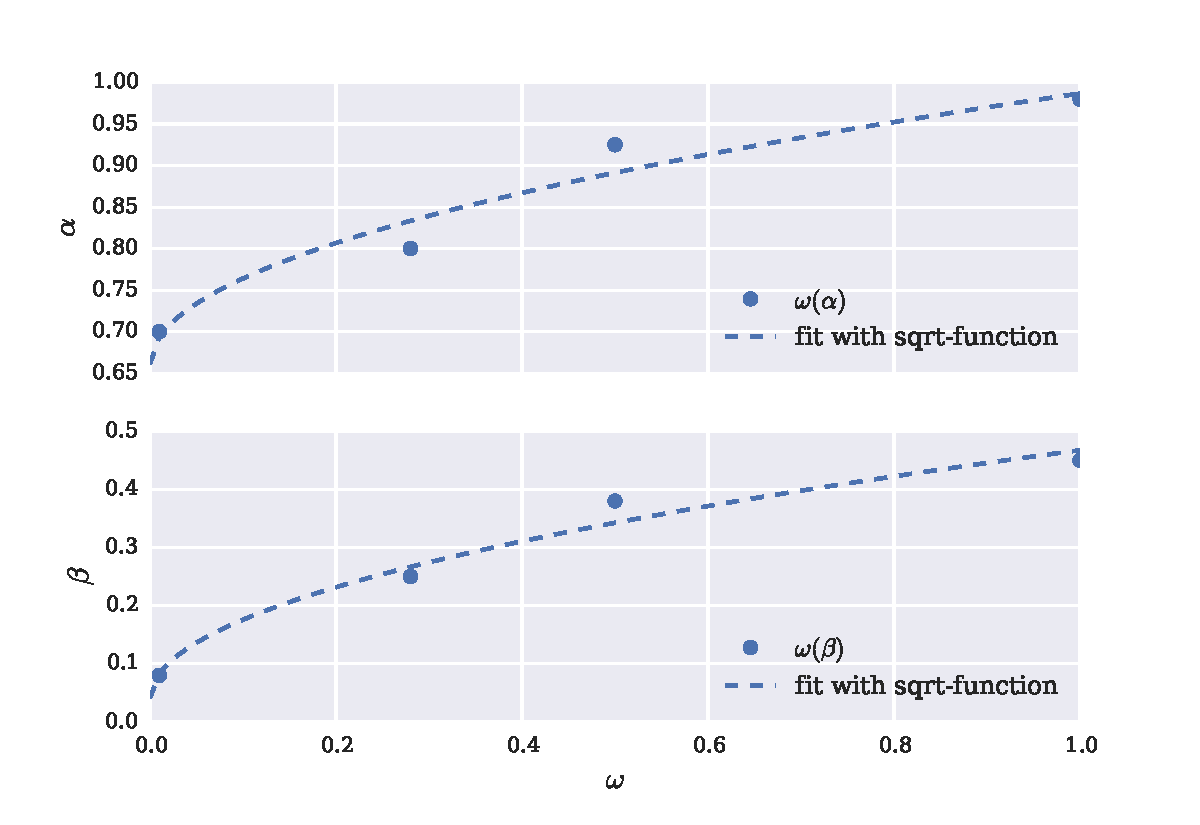
\includegraphics[scale=0.7]{alpha_beta_omega.pdf}
    \caption{Shows the dependency between the locations of the energy minima and the variational parameter. The fit is arbitrary and just to have an orientation which values for $\alpha$ and $\beta$ can be considered in order to reach the energy minimum.}
    \label{fig:alpha_beta_omega}
\end{figure}


All in all our code seems to calculate reliable and good energies. Nevertheless we had to struggle with rather seldom but randomly appearing negative kinetic energies in single cores when using importance sampling. Changing our initial guesses for the starting positions increased here the quality of the solution considerably. In Appendix~\ref{sec:appendix} some three-dimensional plots which show the problem resulting in high energy peaks can be seen. 

\subsubsection{Unperturbed case}
We know that with switched off electron-electron repulsion the lowest energy value should become $10\,\omega$, since we are observing six electrons. In figure \ref{fig:six_electron_unperturbed} this relation is shown for different $\omega$ over $\alpha$ and it can be observed that our results fit very well to the theory. 
\begin{figure}[htbp]
    \centering
    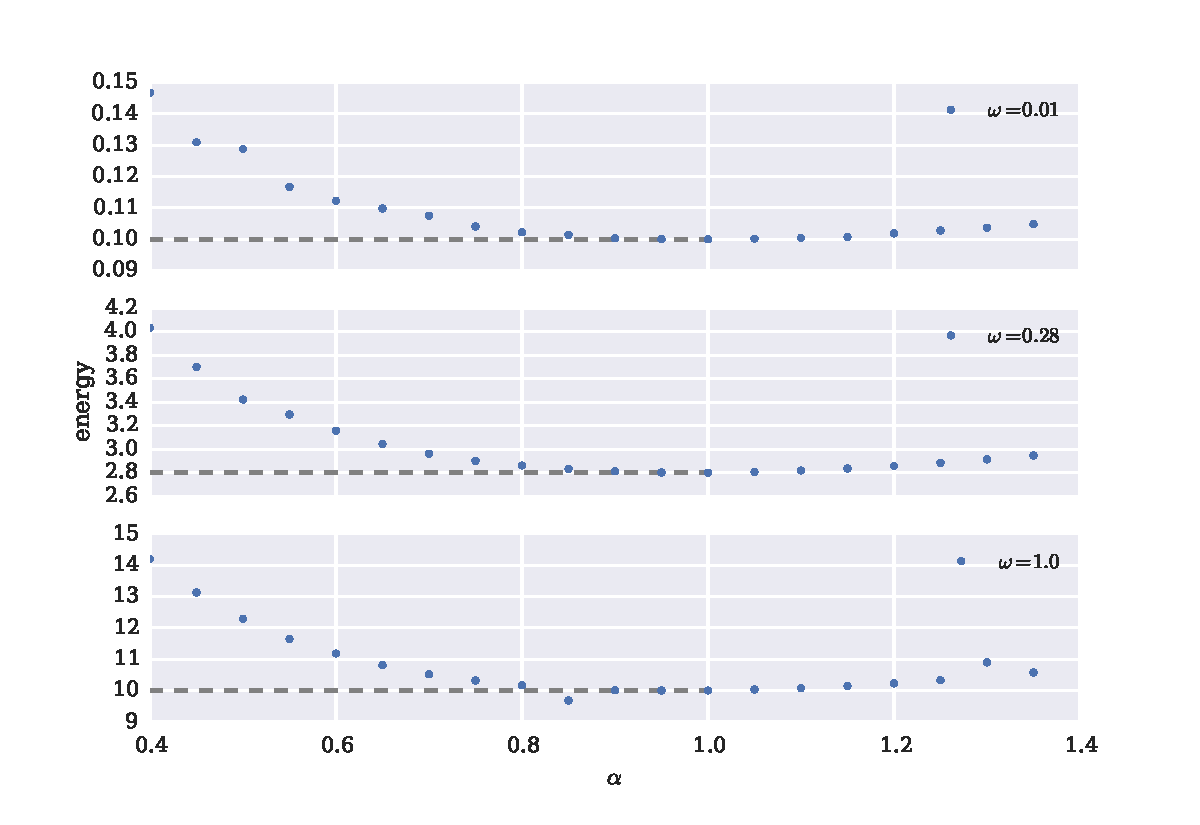
\includegraphics[scale=0.65]{six_electron_unperturbed}
    \caption{The figure shows the energy plotted over the variational parameter $alpha$ assuming six electrons without the repulsive electron-electron forces. For different values of $\omega$ the minimum lies at $10\omega$ which is coherent with the theoretical view.}
    \label{fig:six_electron_unperturbed}
\end{figure}

\subsubsection{Virial theorem}
The virial theorem states a relationship between the mean of the potential $\langle V \rangle$ and of the kinetic energy $\langle T \rangle$ of a closed system. This is described by
\begin{equation}
    \gamma \, \langle V \rangle = 2\, \langle T \rangle,
\end{equation}
with $\gamma$ the homogeneity of the potential $V$. This means for a harmonic oscillator which potential goes with the power of $2$ that one can expect the relationship $\langle V \rangle = \langle T \rangle$. However if we consider the perturbed wavefunction we have additional terms which are stated by the repulsion of the electron and would reveal $\gamma = -1$. Hence, we can make the prediction that the perturbed wavefunction should yield to a smaller ratio 
\begin{equation}
\left(\frac{\langle V \rangle}{\langle T \rangle}\right)_{perturbed} \leq \left(\frac{\langle V \rangle}{\langle T \rangle}\right)_{unperturbed},
\end{equation}
whereas the difference should be larger for smaller $\omega$, because thereby the oscillator potential becomes less relevant. Meanwhile for different $\omega$ and the unperturbed case the ratio should not change and be unity.

In figure \ref{fig:virialtheorem} this behaviour is shown and mostly consistent. Considering first the two electron case we can observe for the unperturbed wavefunction a ratio that is nearly one for all omega. The perturbed part indeed shows the predicted behaviour that it is firstly smaller and secondly it increases with increasing omega. For the six electron system the perturbed functions have the same dependencies as for two electrons with even smaller ratios. This can be physically understood as a more important role for the electron-electron interactions in the six electron case which go with $\gamma = -1$. For the unperturbed part there is a small deviation to unity for larger omegas. This shouldn't be the case and reveals a potential problem in the code for multiple particles. Indeed the data shows that there might be an issue in the draft of the slater matrix. However taking also in reference the known issues of section \ref{sec:perturbed_six} it could also depend on the important sampling. But still after extensive search we were not able to find a malfunction and all other calculations run reasonable, which leads us to the conclusion, that the energies that are produced by our code are reliable values.  
\begin{figure}[htbp]
    \centering
    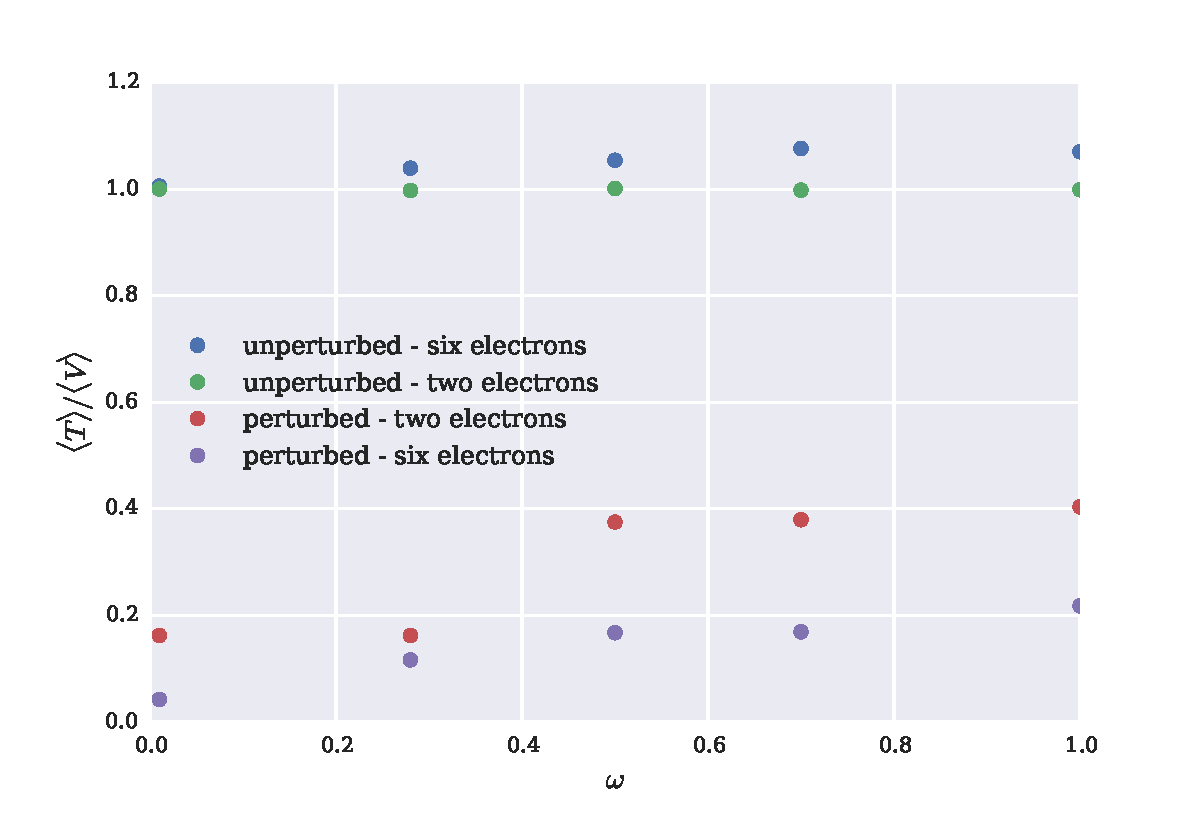
\includegraphics[scale=0.65]{virialtheorem}
    \caption{Shows the fraction of the mean kin. energy $\langle T \rangle$ to the mean pot. energy $\langle V \rangle$ for different values of $\omega$. The calculations are done with either two or six electrons. The unperturbed function}
    \label{fig:virialtheorem}
\end{figure}

\subsection{Closed form solutions}\label{sec:analytical}
Finally we still want to perform calculations with the closed form solutions described in section \ref{sec:closed_form}. For that reason the program was restructured in parts and new classes for the Jastrow-factor and the Slater-matrix including their derivations were introduced. This can be found at the separate branch \texttt{closed\_form} at the provided git repository. The part is fully implemented but unfortunately we were not able to reproduce the solution of the brute force approximations. But still, because we implemented the full code, we are able to examine the time profiling. We thereby used no optimizations yet, like an improved calculation of the inverse slater matrix yet (see \citet{hogberget2013} for more details). An overview for the profiling is given in table \ref{tab:cpu-time}. It was done by calculating $5$ steps with $400000$ cycles on $4$ cores either for $N=2$ or $N=6$ electrons. The time is measured by the linux-command \texttt{time}.
 \begin{table}[htbp]
    \centering
    \caption{CPU-time comparison between closed-form and brute-force measurement}
    \begin{tabular}{c|cc}
    \toprule
    number of electrons   & closed-form    & brute-force   \\
    \midrule
    $2$     & \SI{243.728}{\second}   & \SI{199.636}{\second}  \\
    $6$     & \SI{1448.431}{\second}  & \SI{4779.976}{\second}  \\
    \bottomrule
    \end{tabular}
    \label{tab:cpu-time}
\end{table}

For two electrons it is apparent that the closed-form solution is not faster than the brute-force one. This is probably the case because the evaluation of the wavefunction for only two electrons takes not much time, whereas the calculation of the closed derived formulas inhibits many floating point operations. That the closed-form solution makes sense shows up clearly for six electrons. There the calculation is by a factor of approximately $3.3$ faster, although elaborative calculations like the one of the inverse slater matrix in the equations of section \ref{sec:closed_form} are not stored and evaluated unnecessarily often. Additionally further possible optimizations for the closed-form solution which are not possible in case of the brute force algorithm are not realized. 

